\documentclass[10 pt,usenames,dvipsnames, oneside]{article}
\usepackage{../../modelo-fracoes}
\graphicspath{{../../../Figuras/licao02/}}


\begin{document}

\begin{center}
  \begin{minipage}[l]{3cm}

\includegraphics[width=2cm]{../../../Figuras/logo}       
\end{minipage}\hfill
\begin{minipage}[r]{.8\textwidth}
 {\Large \scshape Atividade: Sete amigos em uma pizzaria rodízio}  
\end{minipage}
\end{center}
\vspace{.2cm}

\ifdefined\prof
\begin{goals}
\begin{enumerate}

    \item       Relembrar divisão com resto (ou divisão euclidiana).
    \item       Selecionar, dentro de uma situação plausível do dia a dia, dados relevantes para resolver um problema.

\end{enumerate}
\tcblower

\begin{itemize} %s
    \item       A atividade deve ser conduzida de forma a chegar-se na divisão euclidiana. Ou seja, o aluno pode começar montando as pizzas. Recomenda-se que os alunos tenham à mão o material concreto: fatias de pizza cortadas em papel ou em E.V.A..
    \item       É possível que os alunos resolvam o item a) a partir da divisão euclidiana, efetuando a divisão de 38 por 8: $38 = 4 \times 8 + 6$. Se esse for o caso, recomenda-se que o professor, destaque a informação associada a cada um dos números na expressão. Em particular, o       ``resto'', que identifica uma quantidade menor do que uma pizza (resto 6 indica 6 fatias, que é menor do que uma pizza, uma vez que cada pizza tem 8 fatias).
    \item       Para responder ao item b), o aluno deve reconhecer que cada fatia é igual a       $\frac{1}{8}$ da pizza. Portanto, a quantidade total de pizza consumida pelos amigos pode ser expressa como       $\frac{38}{8}$ de uma pizza. Cabe destacar que essa fração corresponde a 4 pizzas mais $\frac{6}{8}$ de uma pizza.
    \item        Observe que, neste contexto, o resto, que é um número inteiro e indica o número de fatias, também pode ser expresso por meio de uma fração da unidade pizza:       $\frac{6}{8}$ de uma pizza.
    \item       Faz parte da atividade a tarefa de selecionar dados relevantes para o problema, o que a torna um tanto complexa, por isso é a última Atividade da Lição 2. Para os itens a) e b), a quantidade de amigos, 7, é irrelevante. No entanto, é relevante para o item c).
    \item       A atividade tem também o objetivo de evidenciar que, no cotidiano, nem toda partição é uma equipartição: 38 fatias de pizza para 7 amigos é um exemplo.
\end{itemize} %s

\end{goals}

\bigskip
\begin{center}
{\large \scshape Atividade}
\end{center}
\fi

Em uma pizzaria rodízio, 7 amigos comem, ao todo, 38 fatias.

\begin{center}
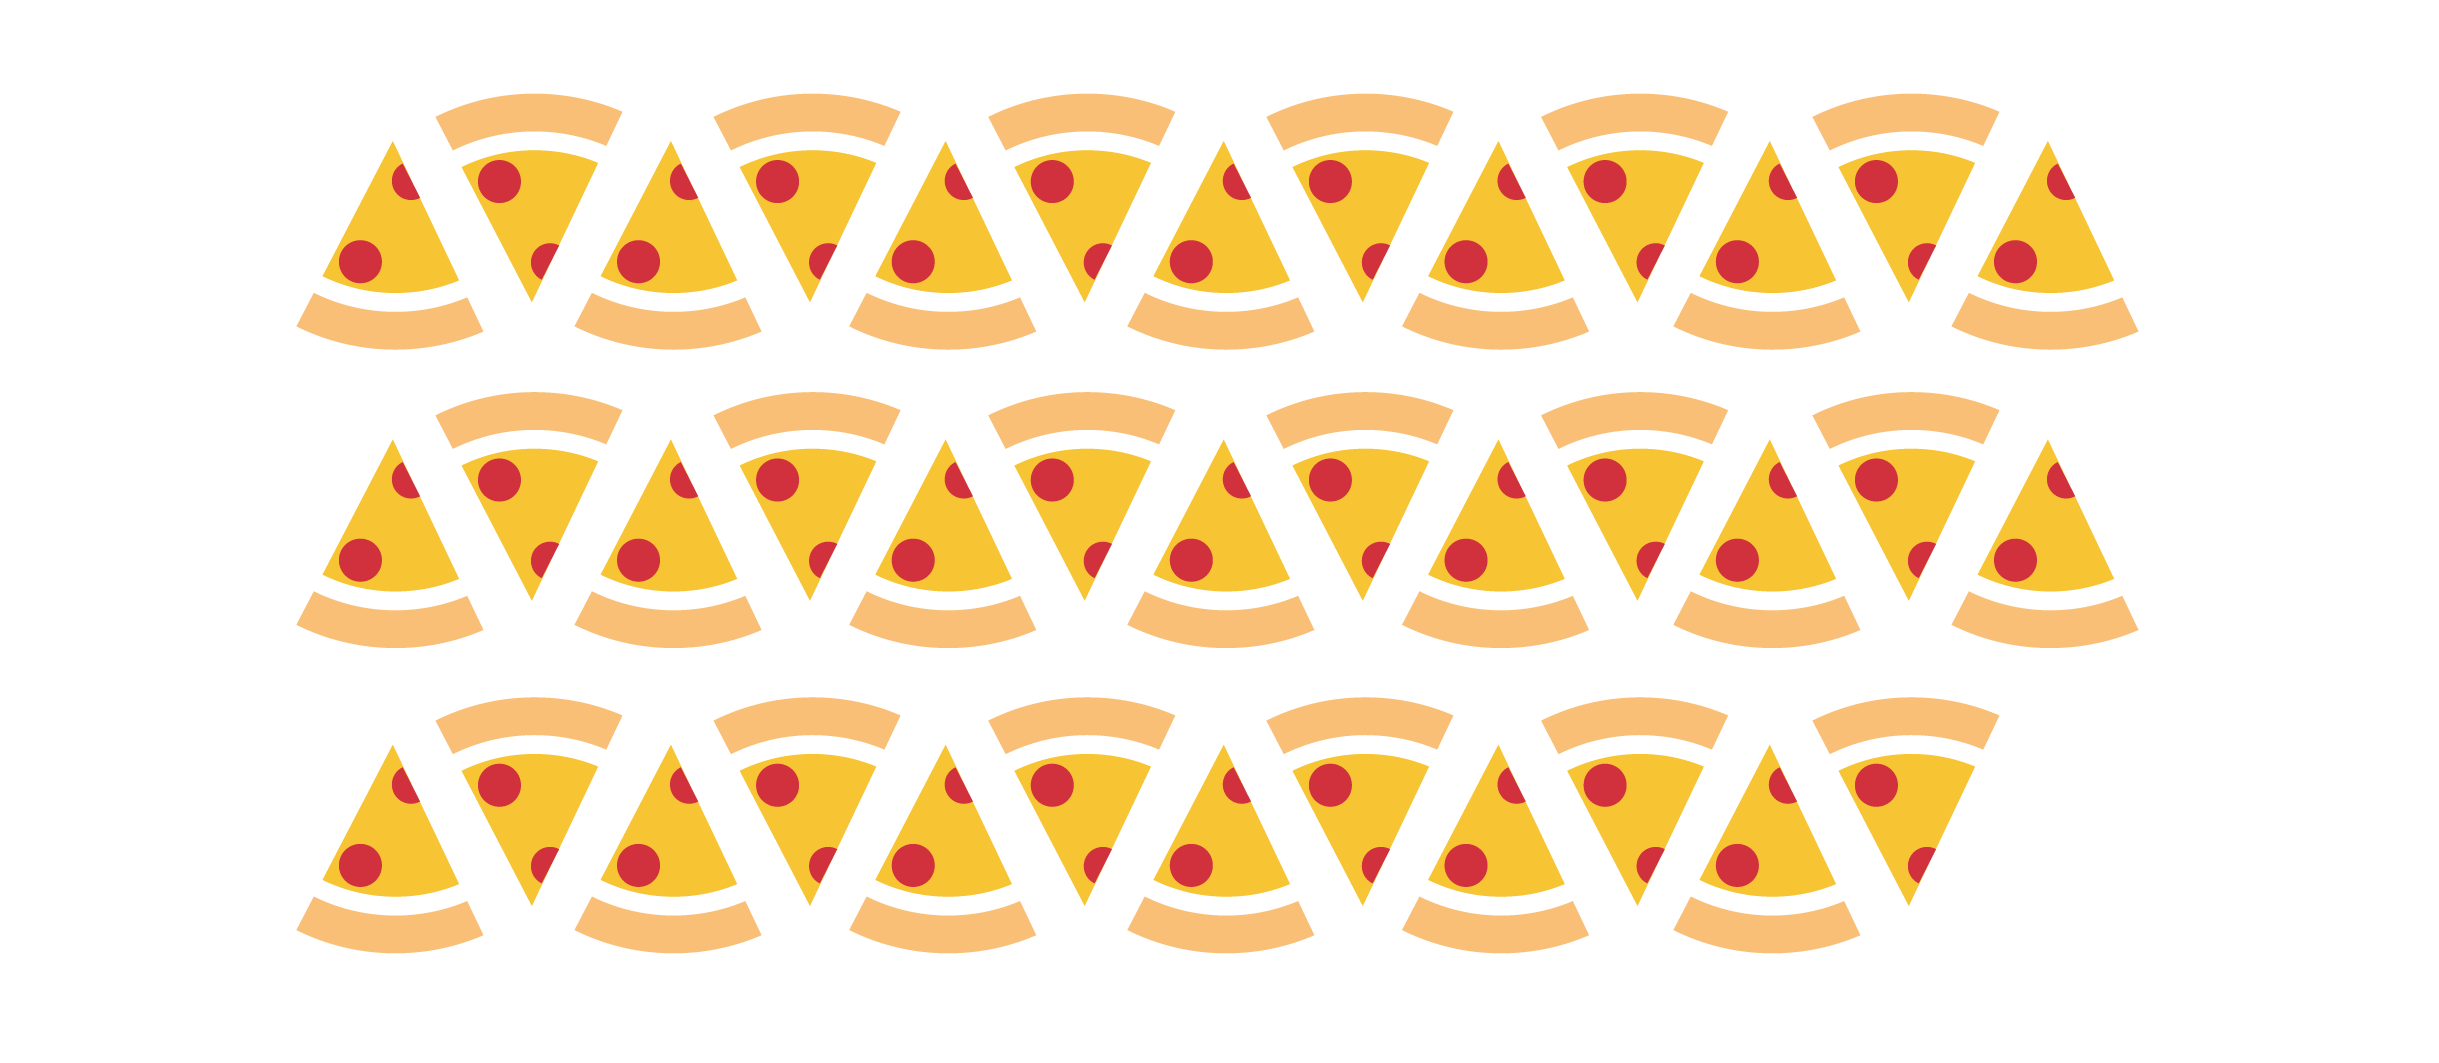
\includegraphics[width=300pt, keepaspectratio]{ativ18_fig01.png}
\end{center}


Sabendo que nessa pizzaria cada pizza é repartida em 8 fatias de mesmo tamanho, pergunta-se:
\begin{enumerate} [label=\alph*)] %s
  \item     Quantas pizzas inteiras comeram os 7 amigos?
  \item     Que fração de uma pizza comeram  ao todo os amigos?
  \item     É possível que todos os amigos tenham comido o mesmo número de fatias de pizza? Explique.
\end{enumerate} %s

\ifdefined\prof

\begin{solucao}


\begin{enumerate} [label=\alph*] %s
    \item       A solução corresponde ao quociente da divisão euclidiana de 38 por 8, ou seja, 4
    \item       Compreendendo que cada fatia é       $\frac{1}{8}$ de uma pizza: 4 pizzas e       $\frac{6}{8}$ ou       $\frac{38}{8}$.
    \item       A divisão euclidiana de 38 por 7 fornece um resto diferente de zero, o que indica que não é possível que todos os amigos tenham comido o mesmo número de fatias de pizza.
\end{enumerate} %s

\end{solucao}
\fi

\end{document}